\documentclass{article}

%usepackages
\usepackage[utf8]{inputenc}
\usepackage{graphicx}
\usepackage[normalem]{ulem}
\usepackage{enumitem}
\usepackage{amsmath}
\usepackage{amssymb}
\usepackage{hyperref}
\usepackage{tikz}
\usepackage[english]{babel}
\usepackage[letterpaper, portrait, margin=1.2in]{geometry}
%\usepackage{fancyhdr}

%new commands
\newcommand{\R}{\mathbb{R}}
\newcommand{\N}{\mathbb{N}}
\newcommand{\Q}{\mathbb{Q}}
\newcommand{\Z}{\mathbb{Z}}
\newcommand{\C}{\mathbb{C}}
\newcommand{\inv}{^{-1}}
\newcommand{\img}{\textmd{Im}\:}
\newcommand{\cok}{\textmd{coker}}
\newcommand{\conv}{\textmd{conv}}
\newcommand{\st}{\textmd{ s.t. }}
\newcommand{\fracfield}{\textmd{frac}\:}

%new theorem environments
\newtheorem{definition}{Definition}[section]
\newtheorem{algodisplay}{Algorithm}[section]
%title
\title{Summary}
\author{Luca Bracone}
%TODO: THIS IS STILL VERY BAREBONES. ADD TEXT BEFORE EVERY SUBSECTION, EXPLAINATION AFTER NN DEFINITION REFERNCING IMAGE. ADD ABSTRACT. THE IMAGE IS IN SPANISH FIND ENGLISH ONE.
\begin{document}
	\maketitle
	\section{Basic Machine Learning}
	\subsection{Neural Networks}
	\begin{definition}[Perceptron]
		A \uline{Perceptron} is a function $ p:\R^n \to \R $ given by 
		\[ p(x_1, \dots , x_n) = g \left( w_0 + \sum_{i=1}^{n} w_i x_i \right)  \]
		Where $ w_1, \dots, w_n \in \R $ are called the \uline{weights} of $p$, $w_0$ is called the \uline{bias}, and $g:\R \to \R $ is any non-linear function called the \uline{activation}.
		Most of the time \[ g(x)=\frac{e^x}{e^x+1} \] the sigmoid function.
	\end{definition}
%	\begin{minipage}{0.3\textwidth}
%			\includegraphics[width=72px]{figure1.png}
%	\end{minipage}
%\begin{minipage}{0.7\textwidth}
	\begin{definition}[Artificial Neural Network]
		A (forward-feeding) \uline{Artificial Neural Network} (ANN) is a function $T: \R^n \to \R^m$ that can be decomposed as such \[ T= l_k \circ \dots \circ l_1  \] Where the $l_i : \R^{n_j} \to \R^{n_{j+1}}$ are called \uline{layers} and are essentially just vectors of perceptrons \[ l_i(\vec{x})=(p_{i,1}(\vec{x}),\dots,p_{i,n_j}(\vec{x})) \].
		In the context of neural networks perceptrons are also called nodes.
	\end{definition}
%\end{minipage}

\begin{definition}[Loss Function]
	For some ANN, $T$ and some input $ (x_1,...,x_n) $, we have a desired output $ (y_1,...,y_n) $ we would like $ T $ to match. Write $ (\hat{y}_1,...,\hat{y}_m) $ the output $T$ actually produced. The \uline{loss} (or sometimes, \uline{cost}) of $T$ for this input is a function that measures the "distance" between the produced and desired output. For most basic applications, 
	\[\mathcal{L}(W; x)= \sum_{i=1}^{m} ||y_i - \hat{y}_i||_2^2  \]
\end{definition}
\begin{definition}[Empirical Loss]
	For a set of inputs $X$, and $T$ a NN, the \uline{Empirical Loss} is 
	\[ J(W)=\frac{1}{|X|} \sum_{\vec{x}\in X} \mathcal{L}(W;x) \]
	the average loss over $X$.
\end{definition}

\subsection{Gradient Descent}
	Any neural network is defined by the weights of its perceptrons. Therefore, in order to have the neural network behave as desired (namely being as close as possible to the desired outputs) we need to find an efficient way to tweak the weights such that the empirical loss becomes as low as possible, when tested on some new inputs. Applying this algorithm repeatedly is called "training".
	\subsubsection{Gradient Descent}
		Essentially it involves taking a step in the "right" direction until we reach a stopping condition, most of the time it's when the steps we are taking are too short. In other words update the weights $W \gets W - \eta \nabla J$. Where $\eta$ is a constant that has to be well chosen. If too small, gradient descent stops when it meets the slightest uphill, and thus misses a better minimum which might be close by. If too big, gradient descent can only take giant steps and diverges to infinity.
	\subsubsection{Gradient Backpropagation}
		In practice, calculating the derivative to some particular weight is quite simple, consider the following neural net: \\ \\
		\begin{minipage}{0.55\linewidth}

		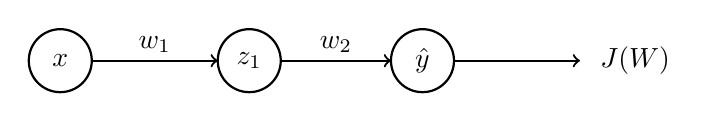
\begin{tikzpicture}
		\draw[thick] (0,0) circle [radius=0.4];
		\node at (0,0) {$x$};
		\draw[->, thick] (0.4,0) -- (2,0);
		\node at (1.2,0.2) {$w_1$};
		\draw[thick] (2.4,0) circle [radius=0.4];
		\node at (2.4,0) {$z_1$};
		\draw[->, thick] (2.8,0) -- (4.2,0);
		\node at (3.5,0.2) {$ w_2 $};
		\draw[thick] (4.6,0) circle [radius=0.4];
		\node at (4.6,0) {$ \hat{y} $};
		\draw[->,thick] (5,0)--(6.6,0);
		\node at (7.3,0) {$ J(W) $};
		\end{tikzpicture}
		\end{minipage}
	\begin{minipage}{0.45\linewidth}
		It's just an application of the chain rule:
		\begin{align*}
		\frac{\partial J}{\partial w_2} &=\frac{\partial J}{\partial \hat{y}} \frac{\partial \hat{y}}{\partial w_2} \\
		\frac{\partial J}{\partial w_1} &= \frac{\partial J}{\partial \hat{y}}\frac{\partial \hat{y}}{\partial z_1}\frac{\partial z_1}{\partial w_1}
		\end{align*}
	\end{minipage}
	\subsubsection{Data Batching}
	Since calculating $\nabla J$ is computationally intensive, consider taking a random subset of your data, and applying gradient descent to it instead. the convergence is going to be more erratic, depending on the size of the subset chosen, but the time gained makes it worth.
	\subsection{Overfitting}
	When training our neural network, it might happen that it essentially "learns the dataset by heart" making it unable to properly tackle on never seen before data points. There are a few methods to avoid such a problem:
		\begin{figure}[ht!]
		\centering
		\includegraphics{overfitting.png}
		\caption[image of overfitting]{A parabola+noise is being misunderstood as a complicated winding line \protect \footnotemark}
		\end{figure}
		\footnotetext{Courtesy of wikimedia foundation \href{https://commons.wikimedia.org/wiki/File:Overfitting.svg}{https://commons.wikimedia.org/wiki/File:Overfitting.svg}}
	\subsubsection{Dropout}
	This technique involves randomly setting some nodes to zero during training. This makes the network not rely too much on some path.
	\subsubsection{Early Stopping}
	After each application of gradient descent, test the network. If it performs worse than it did previously, stop the training process.	
	
	\section{Simplicial Complexes}
	\begin{definition}[convex hull]
	let $ u_0,...,u_k \in \R^n $ their convex hull is
	 \[ \conv \{u_0,...,u_k\} = \left\{ x= \sum_{i=0}^{n} \lambda_i u_i \ \st    \sum_{i=0}^{n} \lambda_i = 1; \ \lambda_i > 0 \ \forall i \right\} \qquad (\star) \]
	\end{definition}
	\begin{definition}[affinitely independent, $k$-simplex]
		$u_0,...,u_k \in \R^n$ are said to be affinitely independent if any point in their convex hull is written as in $(\star)$ uniquely.
		In that case instead of convex hull, we speak of $k$-simplex.
	\end{definition}
	\begin{definition} [face, coface]
		Let $ \{u_{i_0},...,u_{i_m} \} \subseteq \{u_0,...,u_k\} $ we say that $ \tau = \conv\{u_{i_1},...,u_{i_m}\} $ is a face of $ \sigma = \conv\{u_1,..,u_k\} $ which we write $ \tau < \sigma $. Equivalently $ \sigma $ is a coface of $ \tau $.
	\end{definition}
	\begin{definition}[simplicial complex]
		A simplicial complex $K$ is a collection of simplices such that:
		\begin{enumerate}[label=(S\arabic*)]
			\item $ \forall \sigma \in K, \ \tau < \sigma \implies \tau \in K $. 
			\item $ \forall \sigma,\tau \in K, \ \sigma \cap \tau $ is either empty or a face.
		\end{enumerate}
	The dimension of $K$ is $ \dim K = \max_{\sigma \in K} \dim \sigma $ Where the dimension of a $k$-simplex is $k$.
	\end{definition}

\end{document}